
\documentclass[compress]{beamer}

%\usepackage{beamerthemesplit}
\usepackage{xmpmulti}

\usepackage{graphicx,float,wrapfig, bbm}
\usepackage{amsfonts, bbold, comment}
\usepackage{mdwlist}
\usepackage{subfigure}
\usepackage{colortbl}

\usepackage{multirow}

\pgfdeclareimage[width=\paperwidth]{mybackground}{colorado/boulder.pdf}

\newcommand{\e}[2]{\mathbb{E}_{#1}\left[ #2 \right] }
\newcommand{\ind}[1]{\mathbb{I}\left[ #1 \right] }
\newcommand{\ex}[1]{\mbox{exp}\left\{ #1\right\} }
\newcommand{\g}{\, | \,}
\newcommand{\citename}[1]{#1 }

\newcommand{\gfxs}[2]{
\begin{center}
	\includegraphics[width=#2\linewidth]{simtrans/#1}
\end{center}
}

\newcommand{\gfxq}[2]{
\begin{center}
	\includegraphics[width=#2\linewidth]{qb/#1}
\end{center}
}


\usetheme[bullet=circle,                     % Use circles instead of squares for bullets.
          titleline=true,                    % Show a line below the frame title.
          showdate=true,                     % show the date on the title page
          alternativetitlepage=true,         % Use the fancy title page.
          titlepagelogo=general_figures/culogo,              % Logo for the first page.
          % Logo for the header on first page.
          headerlogo=general_figures/boulder_cs,
          ]{UCBoulder}

\usecolortheme{ucdblack}
\title[Thinking on Your Feet]{Thinking on your Feet: \\ \textsc{hsnct} Exhibition Match}
\author{ Jordan Boyd-Graber}
\date{Fall 2014}

\institute[Boulder] % (optional, but mostly needed)
{University of Colorado Boulder}

\AtBeginSection[] % "Beamer, do the following at the start of every section"
{ \begin{frame} \frametitle{Outline} % make a frame titled "Outline"
\tableofcontents[currentsection] % show TOC and highlight current section
\end{frame} }

\begin{document}

\frame{
\titlepage
\tiny
}

\section{Introduction}

\begin{frame}{The Competition}

\begin{itemize}
	\item A computer that plays quiz bowl: \textsc{qanta}
	\item Facing off against four Jeopardy champions
	\pause
	\item But first
	\begin{itemize}
		\item Who we are
		\item How \textsc{qanta} works
		\item Introducing our opponents
	\end{itemize}
	\pause
	\item Afterward: questions and thanks
\end{itemize}

\end{frame}

\section{QANTA}

\begin{frame}
	\frametitle{How is this different from Watson?}

	\begin{columns}
		\column{.5\linewidth}

		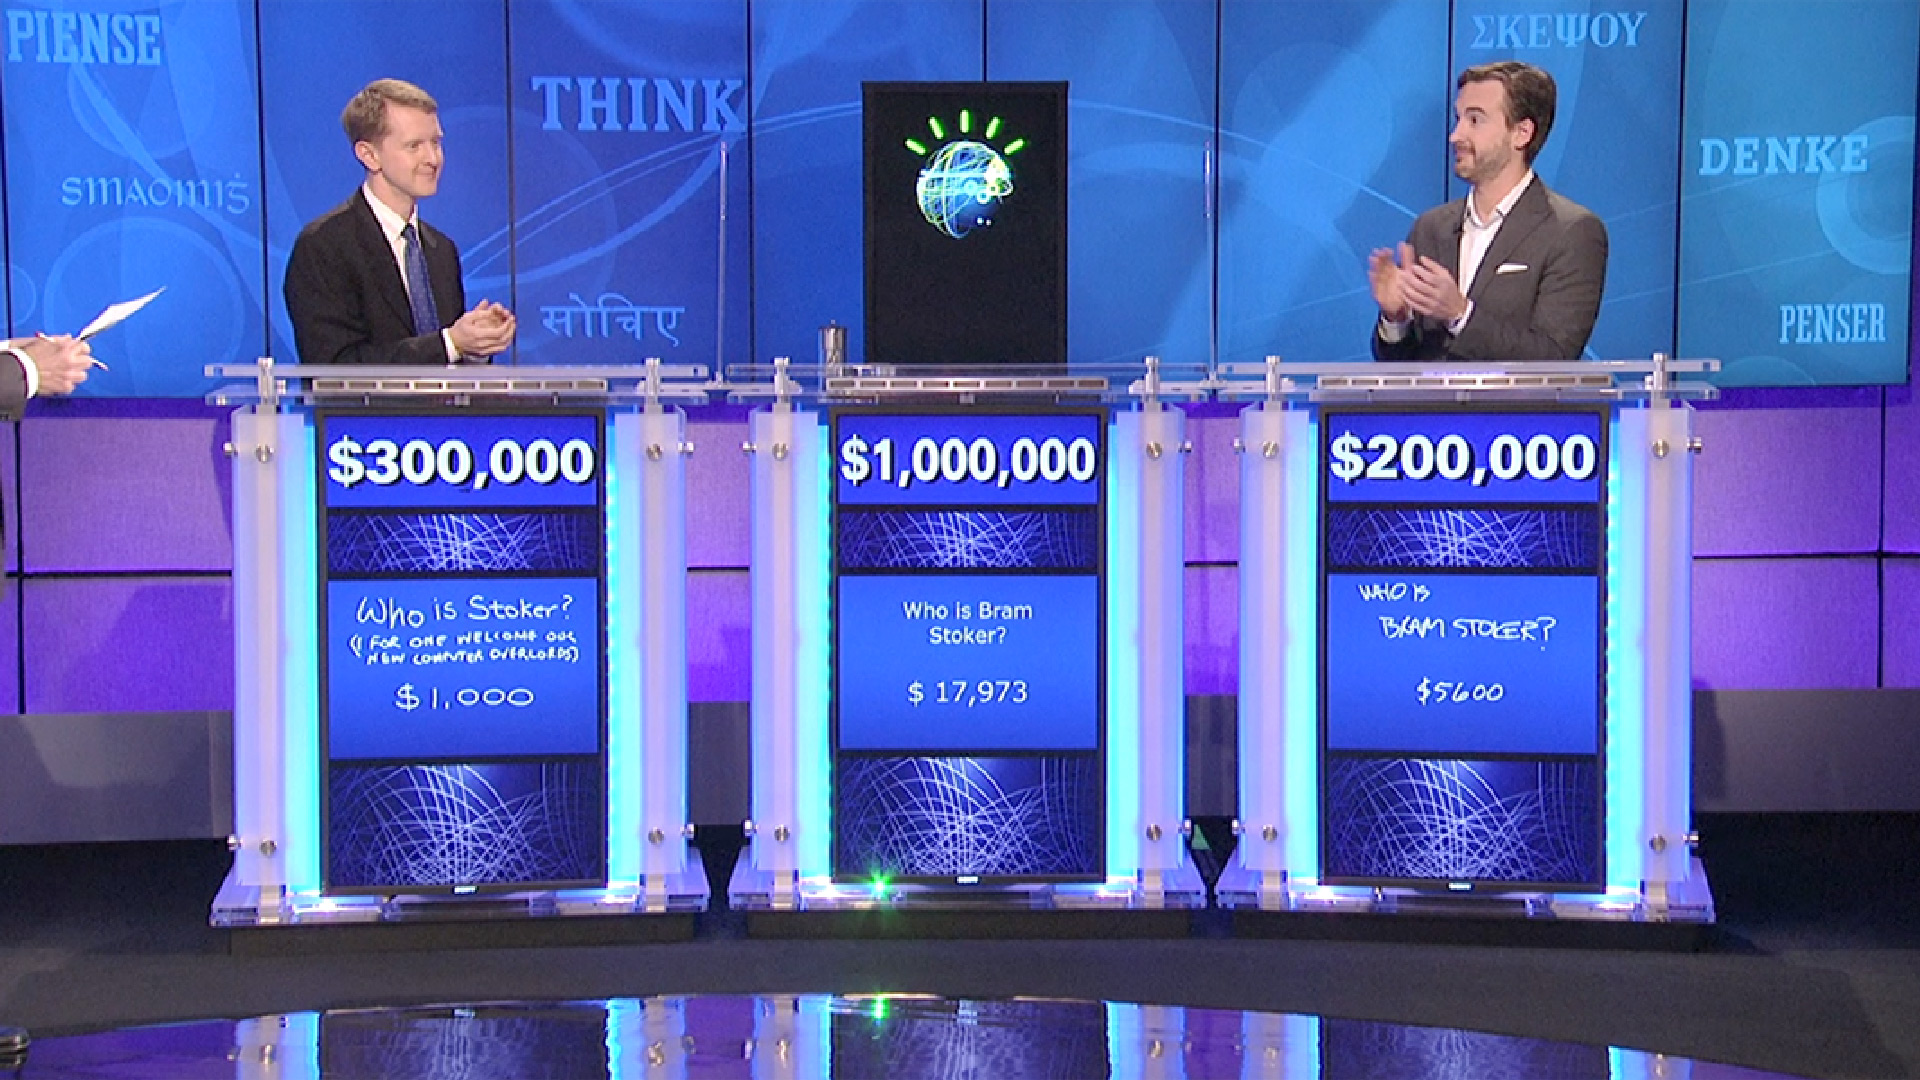
\includegraphics[width=1.0\linewidth]{qb/jeopardy}


		\column{.5\linewidth}
		\begin{itemize}
			\item This is {\bf not} Jeopardy \cite{ferruci-10}
			\item There are buzzers, but players only buzz
                          at the question end
			\item Doesn't discriminate knowledge
			\item Quiz bowl is pyramidal
                        \item Watson must decide to answer {\bf once}, after
                          complete question
                        \item Quiz Bowl: decide after each word
                        \pause
                        \item We're not \textsc{ibm}
		\end{itemize}

	\end{columns}

\end{frame}

\begin{frame}{Who we are}

	\begin{columns}
		\column{.5\linewidth}
			\begin{block}{Jordan Boyd-Graber}
			
			\begin{itemize}
				\item Professor at the University of Colorado
				\item Former quiz bowl player at Caltech (4$^{th}$, 2004 UG ICT) and Princeton (4$^{th}$, ACF Nats 2005)
			\end{itemize}
			
			\end{block}
			\gfxq{jordan_qb}{.5}
		
		
		\column{.5\linewidth}
			\begin{block}{Mohit Iyyer}
			
			\begin{itemize}
				\item Final year PhD student, University of Maryland
				\item National Champion, 2008 HSNCT
			\end{itemize}
			
			\end{block}
			\gfxq{mohit_qb}{.5}	
	\end{columns}

\end{frame}

\section{How QANTA works}

\begin{frame}{Two Steps to Answering Questions}
	Given a question:
	\begin{enumerate}
		\item Generate a set of {\bf guesses} (deep learning)
		\item Select the best guess and {\bf buzz} if confident enough (classifier)
			% \begin{itemize}
			% 	\item Most creative
			% 	\item Can be improved (more later)
			% \end{itemize}
	\end{enumerate}
\end{frame}

\begin{frame}{}

  \begin{columns}
    \column{.4\linewidth}
        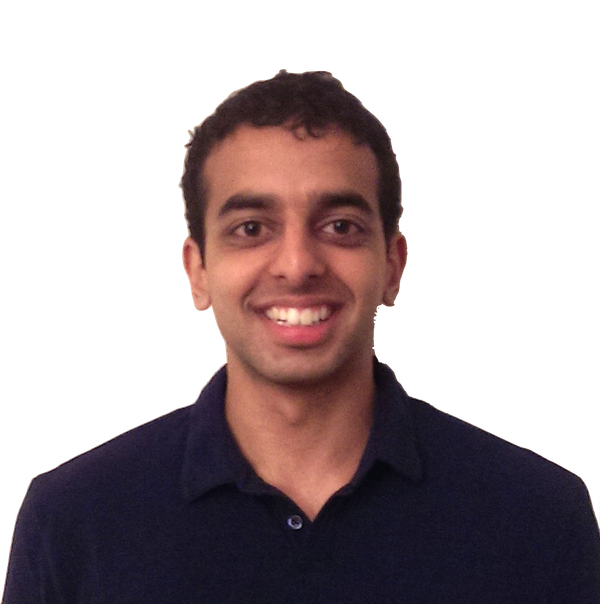
\includegraphics[width=0.9\linewidth]{general_figures/mohit}
    \column{.6\linewidth}
        \begin{block}{ {\bf \href{http://cs.colorado.edu/~jbg//docs/2014_emnlp_qb_rnn.pdf}{A Neural Network for Factoid Question Answering over Paragraphs}}}
\underline{\href{http://cs.umd.edu/~miyyer/}{Mohit Iyyer}}, {\bf Jordan Boyd-Graber}, Leonardo Claudino, Richard Socher, and Hal {Daum\'{e} III}.  \emph{Empirical Methods in Natural Language Processing}, 2014
        \end{block}
        
	\begin{block}{ {\bf \href{http://cs.colorado.edu/~jbg//docs/2015_acl_dan.pdf}{Deep Unordered Composition Rivals Syntactic Methods for Text Classification}} }
	\underline{\href{http://cs.umd.edu/~miyyer/}{Mohit Iyyer}}, {\bf Jordan Boyd-Graber}, and Hal {Daum\'{e} III}.  \emph{Association for Computational Linguistics}, 2015
	
	\end{block}        
        
  \end{columns}
\end{frame}


\begin{frame}{Guesses: Vector Space Model}


  \only<1>{\gfxq{unigram_models_2}{.9}}
  \only<2>{\gfxq{unigram_models_3}{.9}}
  \only<3>{\gfxq{unigram_models_4}{.9}}
  \only<4>{\gfxq{unigram_models_5}{.9}}
  \only<5>{\gfxq{unigram_models_6}{.9}}
  \only<6>{\gfxq{unigram_models_7}{.9}}
  \only<7>{\gfxq{unigram_models_8}{.9}}


\end{frame}

\begin{frame}{Guesses: Vector Space Model}

  \gfxq{embedding}{1.0}

\end{frame}


\begin{frame}{Guesses Example}

	\begin{block}{Question}
	The family sees Stone Mountain and has barbequed sandwiches at The Tower, run by Red Sammy, then heads for Florida over the grandmother's objections.
	\end{block}
	
	\begin{columns}
		\column{.5\linewidth}
		\only<2->{
		\begin{itemize}
			\item Cormac McCarthy
			\item Love in the Time of Cholera
			\item Miguel Angel Asturias
			\item Chronicle of a Death Foretold
			\item \alert<3>{A Good Man Is Hard to Find (short story)}
			\item<2-> {\bf and 195 others!}
		\end{itemize}
		}
		
		\column{.5\linewidth}
		\only<3>{
		The right answer is in this set 80\% of the time.  How do we know which one is right?  And whether we should buzz?}
	\end{columns}

\end{frame}

\begin{frame}{Is a guess right?}

	\begin{columns}
	\column{.75\linewidth}
	\begin{block}{Text}
	The family sees Stone Mountain and has barbequed sandwiches at The Tower, run by Red Sammy, then heads for Florida over the grandmother's objections.
	\end{block}
	\column{.25\linewidth}
	\begin{block}{Guess}
	A Good Man is Hard to Find (short story)
	\end{block}
	\end{columns}
	
	\begin{itemize}
		\item ``Red Sammy'' appears in three questions with this answer and in no other questions
		\item ``grandmother's objections'' appears in the answer's Wikipedia page
		\item The guess does not appear in clues
		\item The question looks like it's about a work
	\end{itemize}
	
	\pause
	
	We use a classifier (Vowpal Wabbit) to decide when to {\bf buzz} or {\bf wait}

\end{frame}

\begin{frame}[t]{Features (by example)}

\only<4->{\vspace{-1.5cm}}

  \begin{columns}[T]
    \column{.3\linewidth}

    \only<1->{ 
\includegraphics[width=2\linewidth]{qb/feature_ex_l_1} \\ }
    \vspace{.5cm}
    \only<4->{ 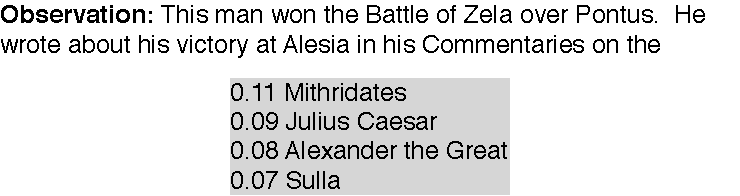
\includegraphics[width=2\linewidth]{qb/feature_ex_l_2}  \\ }
    \vspace{.5cm}
    \only<7->{ 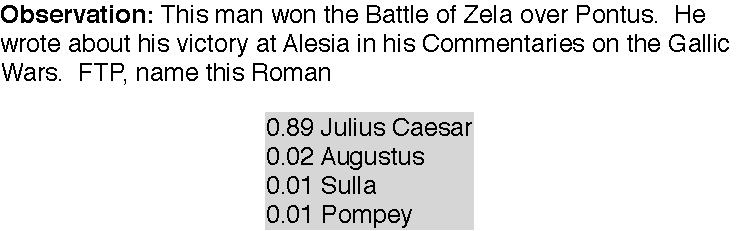
\includegraphics[width=2\linewidth]{qb/feature_ex_l_3}  \\ }


    \column{.68\linewidth}
    \vspace{-.5cm}
    \only<2->{ 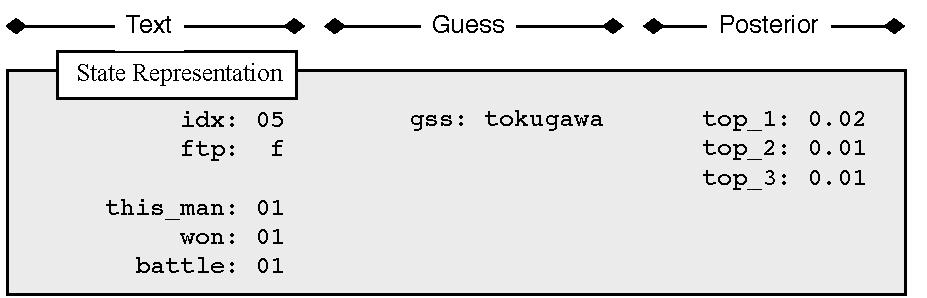
\includegraphics[width=.85\linewidth]{qb/feature_ex_r_1} \\ }
    \only<3->{ \vspace{-.5cm} \hspace{.5cm} 
\includegraphics[width=.1\linewidth]{qb/feature_ex_wait}  \\ }
    \only<5->{ 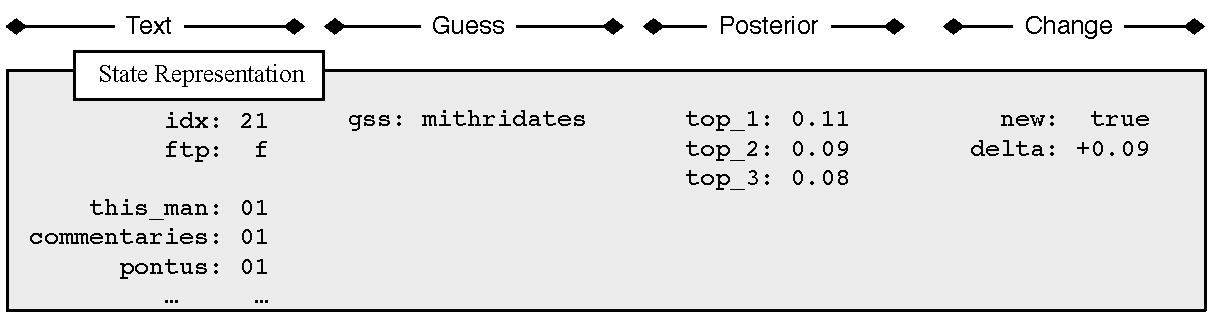
\includegraphics[width=\linewidth]{qb/feature_ex_r_2} \\ }
    \only<6->{ \vspace{-.5cm} \hspace{.5cm}
\includegraphics[width=.1\linewidth]{qb/feature_ex_wait}  \\ }
    \only<8->{ 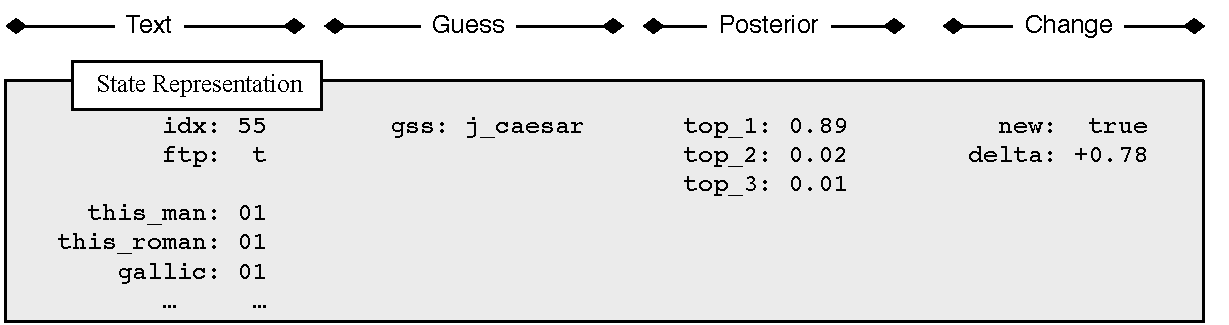
\includegraphics[width=\linewidth]{qb/feature_ex_r_3} \\ }
    \only<9->{ \vspace{-.5cm} \hspace{.5cm} 
\includegraphics[width=.1\linewidth]{qb/feature_ex_buzz}  \\ }
    \only<9->{Answer: {\bf Julius Caesar}}
  \end{columns}

\end{frame}



\begin{frame}{}

  \begin{columns}
    \column{.5\linewidth}
        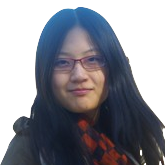
\includegraphics[width=0.9\linewidth]{general_figures/hehe}
    \column{.5\linewidth}
        \begin{block}{{\bf \href{http://cs.colorado.edu/~jbg//docs/qb_emnlp_2012.pdf}{Besting the Quiz Master: Crowdsourcing Incremental Classification Games}}}
          {\bf Jordan Boyd-Graber}, He He, and Hal {Daum\'{e} III}. \emph{Empirical Methods in Natural Language Processing}, 2012
        \end{block}
        
\begin{block}{ {\bf \href{http://cs.colorado.edu/~jbg//docs/2014_emnlp_simtrans.pdf}{Don't Until the Final Verb Wait: Reinforcement Learning for Simultaneous Machine Transl\
ation}}}
\underline{\href{http://www.umiacs.umd.edu/~alvin/}{Alvin Grissom II}}, {\bf Jordan Boyd-Graber}, He He, John Morgan, and Hal {Daum\'{e} III}.  \emph{Empirical Methods in Natural L\
anguage Processing}, 2014
        \end{block}        
  \end{columns}
\end{frame}



\begin{frame}
\frametitle{How do we know if we're doing well?}

\begin{columns}

	\column{0.5\linewidth}

	\begin{center}
		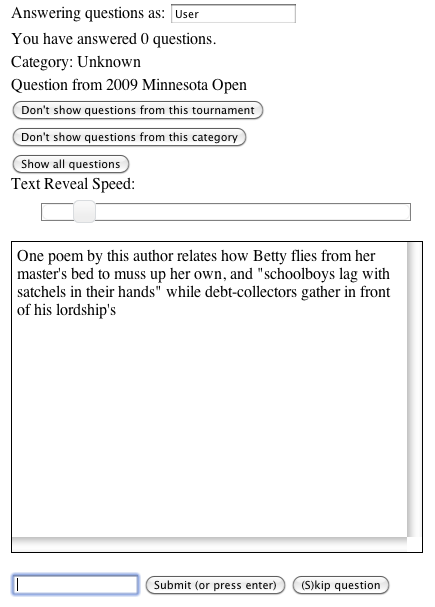
\includegraphics[width=0.8\linewidth]{qb/screenshot}
	\end{center}

	\column{0.5\linewidth}

	\begin{itemize}
		\item 2010: Website where people could play quiz bowl online
		\item 7000 questions were answered in the first day
		\item Over 43000 questions were answered in the space of two weeks
		\item Total of 461 unique users
		\item Leaderboard to encourage users
		\pause
		\item Progenitor of ProtoBowl
	\end{itemize}

\end{columns}
\end{frame}


\begin{frame}{Now we're able to beat humans}

  \gfxq{human_history}{1.0}
  \pause
  
 Until today, our system has never faced an opponent face to screen

\end{frame}


\section{Competition}

\begin{frame}{What's next}

	\begin{itemize}
		\item 40 questions from rounds 15 \& 16
		\item No bonuses
		\item \textsc{qanta} sees a word when I push a button: decides when to answer
		\item Mohit will input whether players are correct or not
		\pause
		\item Our opponents
		\begin{columns}
			\column{.25\linewidth}
				\gfxq{colby_jeo}{1.0}
			\column{.25\linewidth}
				\gfxq{ben_jeo}{1.0}
			\column{.25\linewidth}
				\gfxq{alex_jeo}{1.0}
			\column{.25\linewidth}
				\gfxq{kristin_jeo}{1.0}						
		\end{columns}
	\end{itemize}

\end{frame}


\begin{frame}{Why simultaneous translation hard is}

  \begin{columns}
    \column{.5\linewidth}
       \gfxs{nuremberg_translators}{.9}
    \column{.5\linewidth}
       \begin{itemize}
         \item Languages like German and Japanese are {\bf verb final}
         \item Simultaneous translation requires you to think on your feed
         \item Predict when you know the verb so you can translate to English
       \end{itemize}
  \end{columns}

\end{frame}

\begin{frame}{Questions and Discussion}

	\begin{center}
	\begin{Huge}
	?
	\end{Huge}
	\end{center}

\end{frame}


\begin{frame}{Postmortem}

\begin{itemize}
	\item Only most common 4,000 answers
	\item Trash and current events: too much churn
	\item Creative questions
	\item Common link questions
	\item Before and after
	\item Wordplay
	\item Computation
\end{itemize}


\end{frame}

\begin{frame}{We want (and need) your help!}

	\begin{itemize}
		\item Our system isn't perfect
		\item We need more data
		\item We need more features
		\item We need excellent coders	
	\end{itemize}
	
	\pause

	\begin{block}{Find out more \dots}
		\begin{itemize}
			\item Code: \url{http://github.com/miyyer/qb}
			\item Twitter: @boydgraber
			\item Announcements on HSQB
		\end{itemize}
	\end{block}

\end{frame}

\begin{frame}{Come to Boulder}

\begin{columns}
	\column{.5\linewidth}
        \only<1>{
        	\begin{center}
		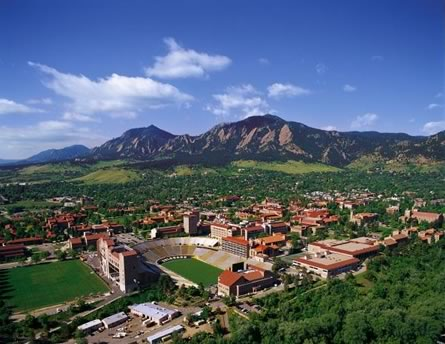
\includegraphics[width=.9\linewidth]{colorado/boulder} \\
		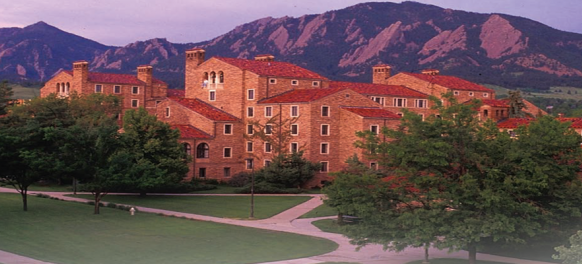
\includegraphics[width=.9\linewidth]{colorado/cs_dept}
	\end{center}
              }
	\column{.5\linewidth}	
		\begin{itemize}
			\item Looking for undergrads/grads/interns to combine cutting edge artificial intelligence with trivia
			\item One of the best schools for natural language processing in the world
		\end{itemize}
\end{columns}

\end{frame}


\frame{

	\frametitle{Thanks}

        \begin{block}{Collaborators}
          \textsc{naqt}, Hal Daum\'e III (UMD), Anupam Guha (Maryland), Manjhunath Ravi (Colorado), Danny Bouman (UMD UG),
          Stephanie Hwa (UMD UG)
        \end{block}

	\begin{columns}
	
	\column{.45\linewidth}
        \begin{block}{Funders}
        \begin{center}
          
\includegraphics[width=0.4\linewidth]{general_figures/nsf}
       \end{center}
        \end{block}
        
        \pause
	\column{.45\linewidth}        
        \begin{block}{Supporters}
        	\gfxq{naqt}{.4}
        \end{block}
        
        \end{columns}
}



\begin{frame}{References}
\bibliographystyle{style/acl}
\tiny
\bibliography{bib/journal-full,bib/jbg}
\end{frame}




	%

\begin{frame}
	\frametitle{Learning which Features are Useful}

	\begin{itemize}
		\item Use how humans these data as a prior for supervised maxent model~\cite{daume-04}
		\item Prior for label $a$ and feature $f$ is a function of the number of buzzes $b$ and tf-idf~\cite{salton-68}
\begin{equation}
  \left[ \vphantom{\frac{a}{b}}\alpha \alert<4>{\ind{ b(a,f) > 0}} + \beta \alert<3>{ b(a,f)} + \gamma
  \right] \alert<2>{\mbox{tf-idf}(a,f)} .
\label{eq:meanweight}
\end{equation}
		\begin{itemize}
			\item $\alpha$, $\beta$, and $\gamma = 0$: na\"ive zero prior
			\item $\alpha$ and $\beta = 0$: linear transformation of the mean
			\item $\alpha$ and $\gamma = 0$: number of buzzes times tf-idf value of the features
		\end{itemize}

	\end{itemize}

\end{frame}

\begin{frame}
	\frametitle{Using buzzes as a prior}

\begin{equation*}
  \left[ \vphantom{\frac{a}{b}}\alpha \ind{ b(a,f) > 0} + \beta b(a,f) + \gamma
  \right] \mbox{tf-idf}(a,f) .
\end{equation*}

\begin{center}
\begin{tabular}{cccccc}
Answers & Weighting & $\alpha$ & $\beta$ & $\gamma$ & Error\footnote{Buzz and tf-idf computed on training data; grid search on dev data; error on test data} \\
\hline
\multirow{5}{*}{100} & zero & - & - & - & 0.22 \\
& tf-idf & - & - & 8.3 & 0.08 \\
&  buzz-binary & 10.7 & - & - & {\bf 0.06} \\
&  buzz-linear & - &  1.1 & - & 0.10 \\
& buzz-tier & - & 1.6 & 0.5 & 0.07 \\
\hline
\end{tabular}
\end{center}
\end{frame}





\begin{frame}
	\begin{center}

\vspace{-.6cm}
\begin{figure}[tb]
\centering

\subfigure[Buzzes over all Questions]{
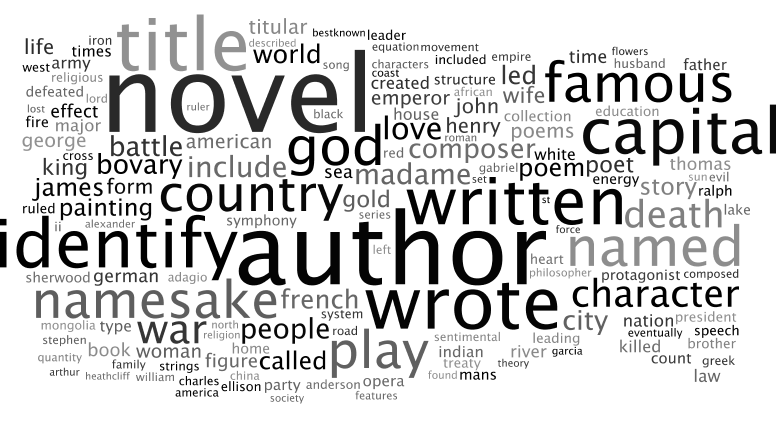
\includegraphics[width=0.6\linewidth]{qb/buzz_cloud}
\label{fig:buzz_cloud}
}

\subfigure[Wuthering Heights Question Text]{
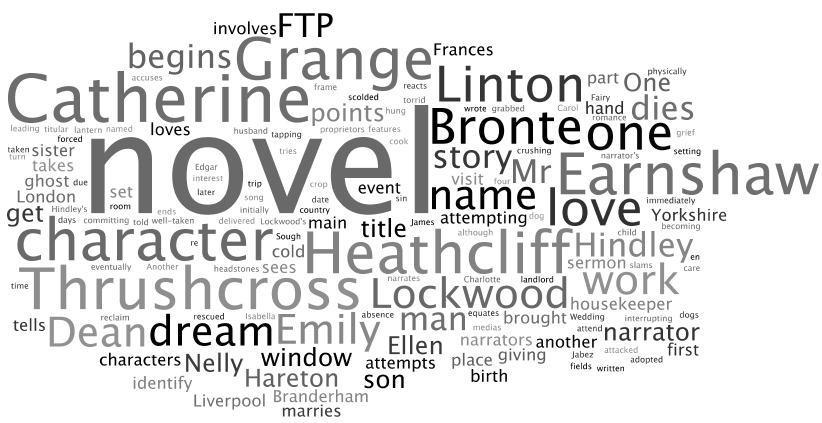
\includegraphics[width=0.45\linewidth]{qb/wuthering_heights_question}
\label{fig:wh_question}
}
\subfigure[Buzzes on Wuthering Heights]{
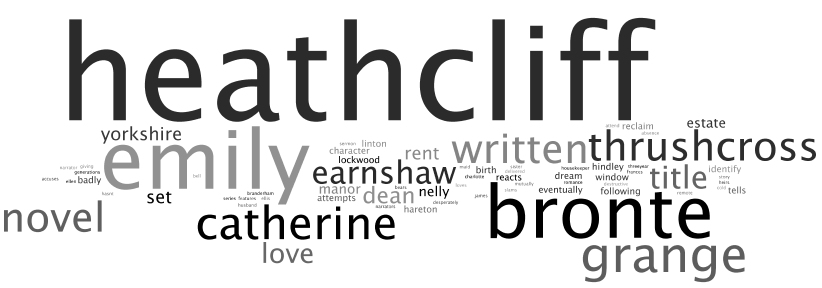
\includegraphics[width=0.45\linewidth]{qb/wuthering_heights_buzz}
\label{fig:wh_buzz}
}
\end{figure}


	\end{center}

\end{frame}



\begin{frame}
	\frametitle{Accuracy vs. Speed}

	\begin{center}
	  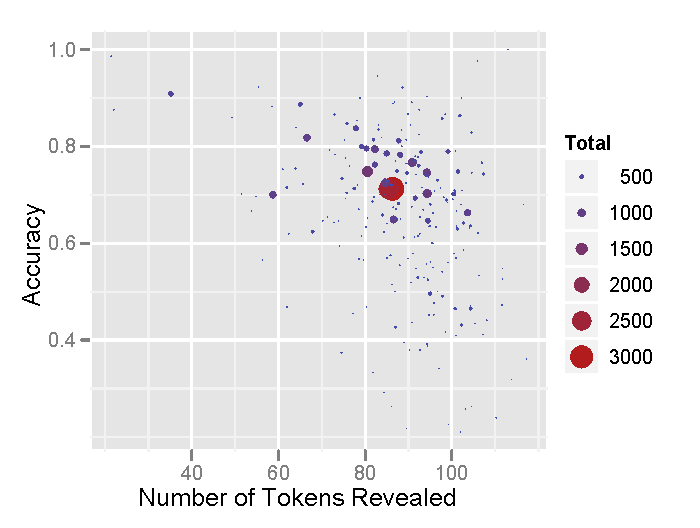
\includegraphics[width=0.8\linewidth]{qb/accuracy_vs_speed}
	  \end{center}

\end{frame}




\end{document}
